Right now, as you read this, particles are passing through your body at nearly the speed of light. Roughly one muon traverses each square centimeter of your skin every minute. They originate 10–20 kilometers above Earth's surface, born from collisions between cosmic rays and atmospheric nuclei. They rain down continuously, penetrating buildings, mountains, and human tissue, leaving faint trails of ionization as they pass.

What is a muon? It belongs to a family of particles called leptons — point-like matter particles that do not experience the strong nuclear force. The most familiar lepton is the electron, which orbits atomic nuclei and carries electric current through wires. The muon is essentially a heavier version of the electron: same electric charge ($-1$), same spin ($\tfrac{1}{2}$), but 207 times more massive at $105.7\,\text{MeV}/c^2$. This extra mass makes the muon unstable. It decays via the weak interaction:
\[
\mu^- \rightarrow e^- + \bar{\nu}_e + \nu_\mu
\]
producing an electron and two neutrinos. Laboratory measurements show this decay occurs with a mean lifetime of 2.2 microseconds in the muon's rest frame.

Atmospheric muons begin with cosmic rays — mostly high-energy protons accelerating through interstellar space, some reaching energies up to $10^{11}$ GeV. When these protons strike atmospheric nuclei at altitudes of 10–20 kilometers, they produce hadronic showers: cascades of secondary particles including pions and kaons. Pions decay rapidly:
\[
\pi^+ \rightarrow \mu^+ + \nu_\mu, \qquad \pi^- \rightarrow \mu^- + \bar{\nu}_\mu
\]
with a rest-frame lifetime of 26 nanoseconds. Because the pions travel at relativistic speeds, their decay products inherit high energies and directionality. The resulting muons typically have energies of 1–10 GeV and velocities exceeding $0.995c$.

Here lies the puzzle. A muon at rest lives 2.2 microseconds. Even traveling at light speed, this permits a maximum distance of:
\[
d_{\text{classical}} = c \cdot \tau_0 = 3 \times 10^8\,\text{m/s} \cdot 2.2 \times 10^{-6}\,\text{s} \approx 660\,\text{m}
\]
Classical physics predicts that muons created 15 kilometers up should decay long before reaching sea level. Detectors at ground level should register only a tiny residual flux — the rare survivors from production events occurring just above the stratosphere.

But measurements show otherwise. Muons arrive at sea level in abundance, approximately one per square centimeter per minute. Some penetrate deep underground, detected in mines and beneath mountains. The observed flux exceeds classical predictions by more than an order of magnitude. If Newtonian mechanics governed particle decay, atmospheric muons would be rare curiosities, not the dominant component of cosmic radiation at Earth's surface.

Special relativity resolves the paradox. From Earth's reference frame, the muon's lifetime dilates according to the Lorentz factor:
\[
\tau_{\text{observed}} = \gamma \tau_0, \qquad \gamma = \frac{1}{\sqrt{1 - v^2/c^2}}
\]
For a muon traveling at $v = 0.998c$, we calculate $\gamma \approx 15$. The observed lifetime extends to:
\[
\tau_{\text{observed}} = 15 \times 2.2\,\mu\text{s} \approx 33\,\mu\text{s}
\]
allowing the muon to cover approximately 10 kilometers before decaying. This matches the observed sea-level flux and explains detections deep underground.

From the muon's rest frame, time passes normally — it still lives only 2.2 microseconds by its own clock. But the atmosphere is contracted along the direction of motion by the same factor $\gamma$. The 15-kilometer journey from production altitude to sea level contracts to roughly 1 kilometer in the muon's frame. This distance is easily traversable within 2.2 microseconds at $0.998c$. Both perspectives yield identical predictions: muons reach sea level. The symmetry reflects the covariance of physical laws under Lorentz transformations — no preferred reference frame exists.

Detecting muons exploits their electric charge and penetrating power. As they traverse matter, they ionize atoms along their path, losing energy gradually. Unlike electrons, which radiate intensely at high energies (bremsstrahlung), muons are massive enough to suppress radiative losses. They pass through meters of rock or steel with only modest energy attenuation.

The simplest detector uses a scintillator — a material that emits light when ionized — coupled to a photomultiplier tube. When a muon passes through, it excites molecules in the scintillator, which promptly re-emit photons. The photomultiplier amplifies this signal into a measurable electrical pulse. Cloud chambers and bubble chambers reveal muon tracks visually: the particle ionizes a supersaturated or superheated medium, leaving a trail of condensation or bubbles. Modern experiments use arrays of scintillation counters, drift chambers, or resistive plate chambers with timing electronics to reconstruct trajectories and measure momenta.

At sea level, the vertical muon flux is approximately one per square centimeter per minute, with typical energies around 4 GeV. This makes muons the dominant component of secondary cosmic radiation at Earth's surface. They contribute background signals in neutrino detectors, serve as calibration sources for particle physics experiments, and enable muon tomography — a radiographic technique that uses atmospheric muons to image dense structures like nuclear reactor cores or hidden chambers in pyramids.

The atmospheric muon flux provided one of the earliest natural confirmations of relativistic time dilation. The phenomenon requires no synchronized atomic clocks, no particle accelerators, no carefully orchestrated experimental setup. Nature performs the test constantly. Bruno Rossi and David Hall's 1941 measurements, comparing muon counts at different altitudes, demonstrated quantitative agreement with relativistic predictions. The data matched time dilation calculations and ruled out classical decay rates.

This test carries philosophical weight. Skeptics might argue that relativistic formulas are mathematical conveniences — useful calculational tools with no physical reality. Atmospheric muons refute this: particles created at high altitude, traveling macroscopic distances through the atmosphere, reach ground-level detectors in numbers precisely predicted by relativistic kinematics. The agreement between laboratory measurements of rest-frame decay rates and atmospheric propagation distances over tens of kilometers confirms that time dilation is not an artifact of coordinate systems but a physical consequence of spacetime geometry.

The muon's place within the Standard Model reveals a deeper puzzle. Fundamental matter particles divide into two families: quarks, which carry color charge and form composite hadrons like protons and neutrons, and leptons, which are point-like and unaffected by the strong nuclear force. The six known leptons arrange into three generations:
\begin{itemize}
\item First generation: electron ($e^-$), electron neutrino ($\nu_e$)
\item Second generation: muon ($\mu^-$), muon neutrino ($\nu_\mu$)
\item Third generation: tau ($\tau^-$), tau neutrino ($\nu_\tau$)
\end{itemize}

Each generation replicates the pattern: one charged lepton and one neutral neutrino. The charged leptons have identical electric charge and spin but vastly different masses. The electron at $0.511\,\text{MeV}/c^2$ is stable. The muon, 207 times heavier, decays in 2.2 microseconds. The tau lepton, at $1776.9\,\text{MeV}/c^2$, survives only 290 femtoseconds. Neutrinos have no electric charge, interact only via the weak force and gravity, and possess extremely small masses — each less than $1\,\text{eV}/c^2$.

Quarks mirror this generational structure: up and down (first generation), charm and strange (second), top and bottom (third). Each generation preserves the same interaction patterns and quantum numbers, differing only in mass and lifetime. Heavier fermions decay into lighter ones through weak interactions, conserving energy, momentum, and quantum numbers.

Why three generations? The Standard Model incorporates this structure through input parameters — masses, mixing angles, decay constants — but offers no explanation for the number of generations or the mass hierarchy. The replication appears arbitrary. Nothing in gauge theory or quantum field theory requires precisely three generations, yet all known fermions fit this pattern. The muon, when first discovered, seemed superfluous — physicist Isidor Rabi's quip "Who ordered that?" captured the bewilderment. It plays no obvious role in atomic structure or nuclear processes, yet it exists, precisely replicating the electron's quantum numbers at a different mass scale.

The generational structure affects everything from CP violation in weak decays to neutrino oscillations to the running of coupling constants at high energies. But the underlying reason — why nature chose three generations, why the mass ratios span orders of magnitude — remains unknown.

\begin{center}
\vspace*{2em}
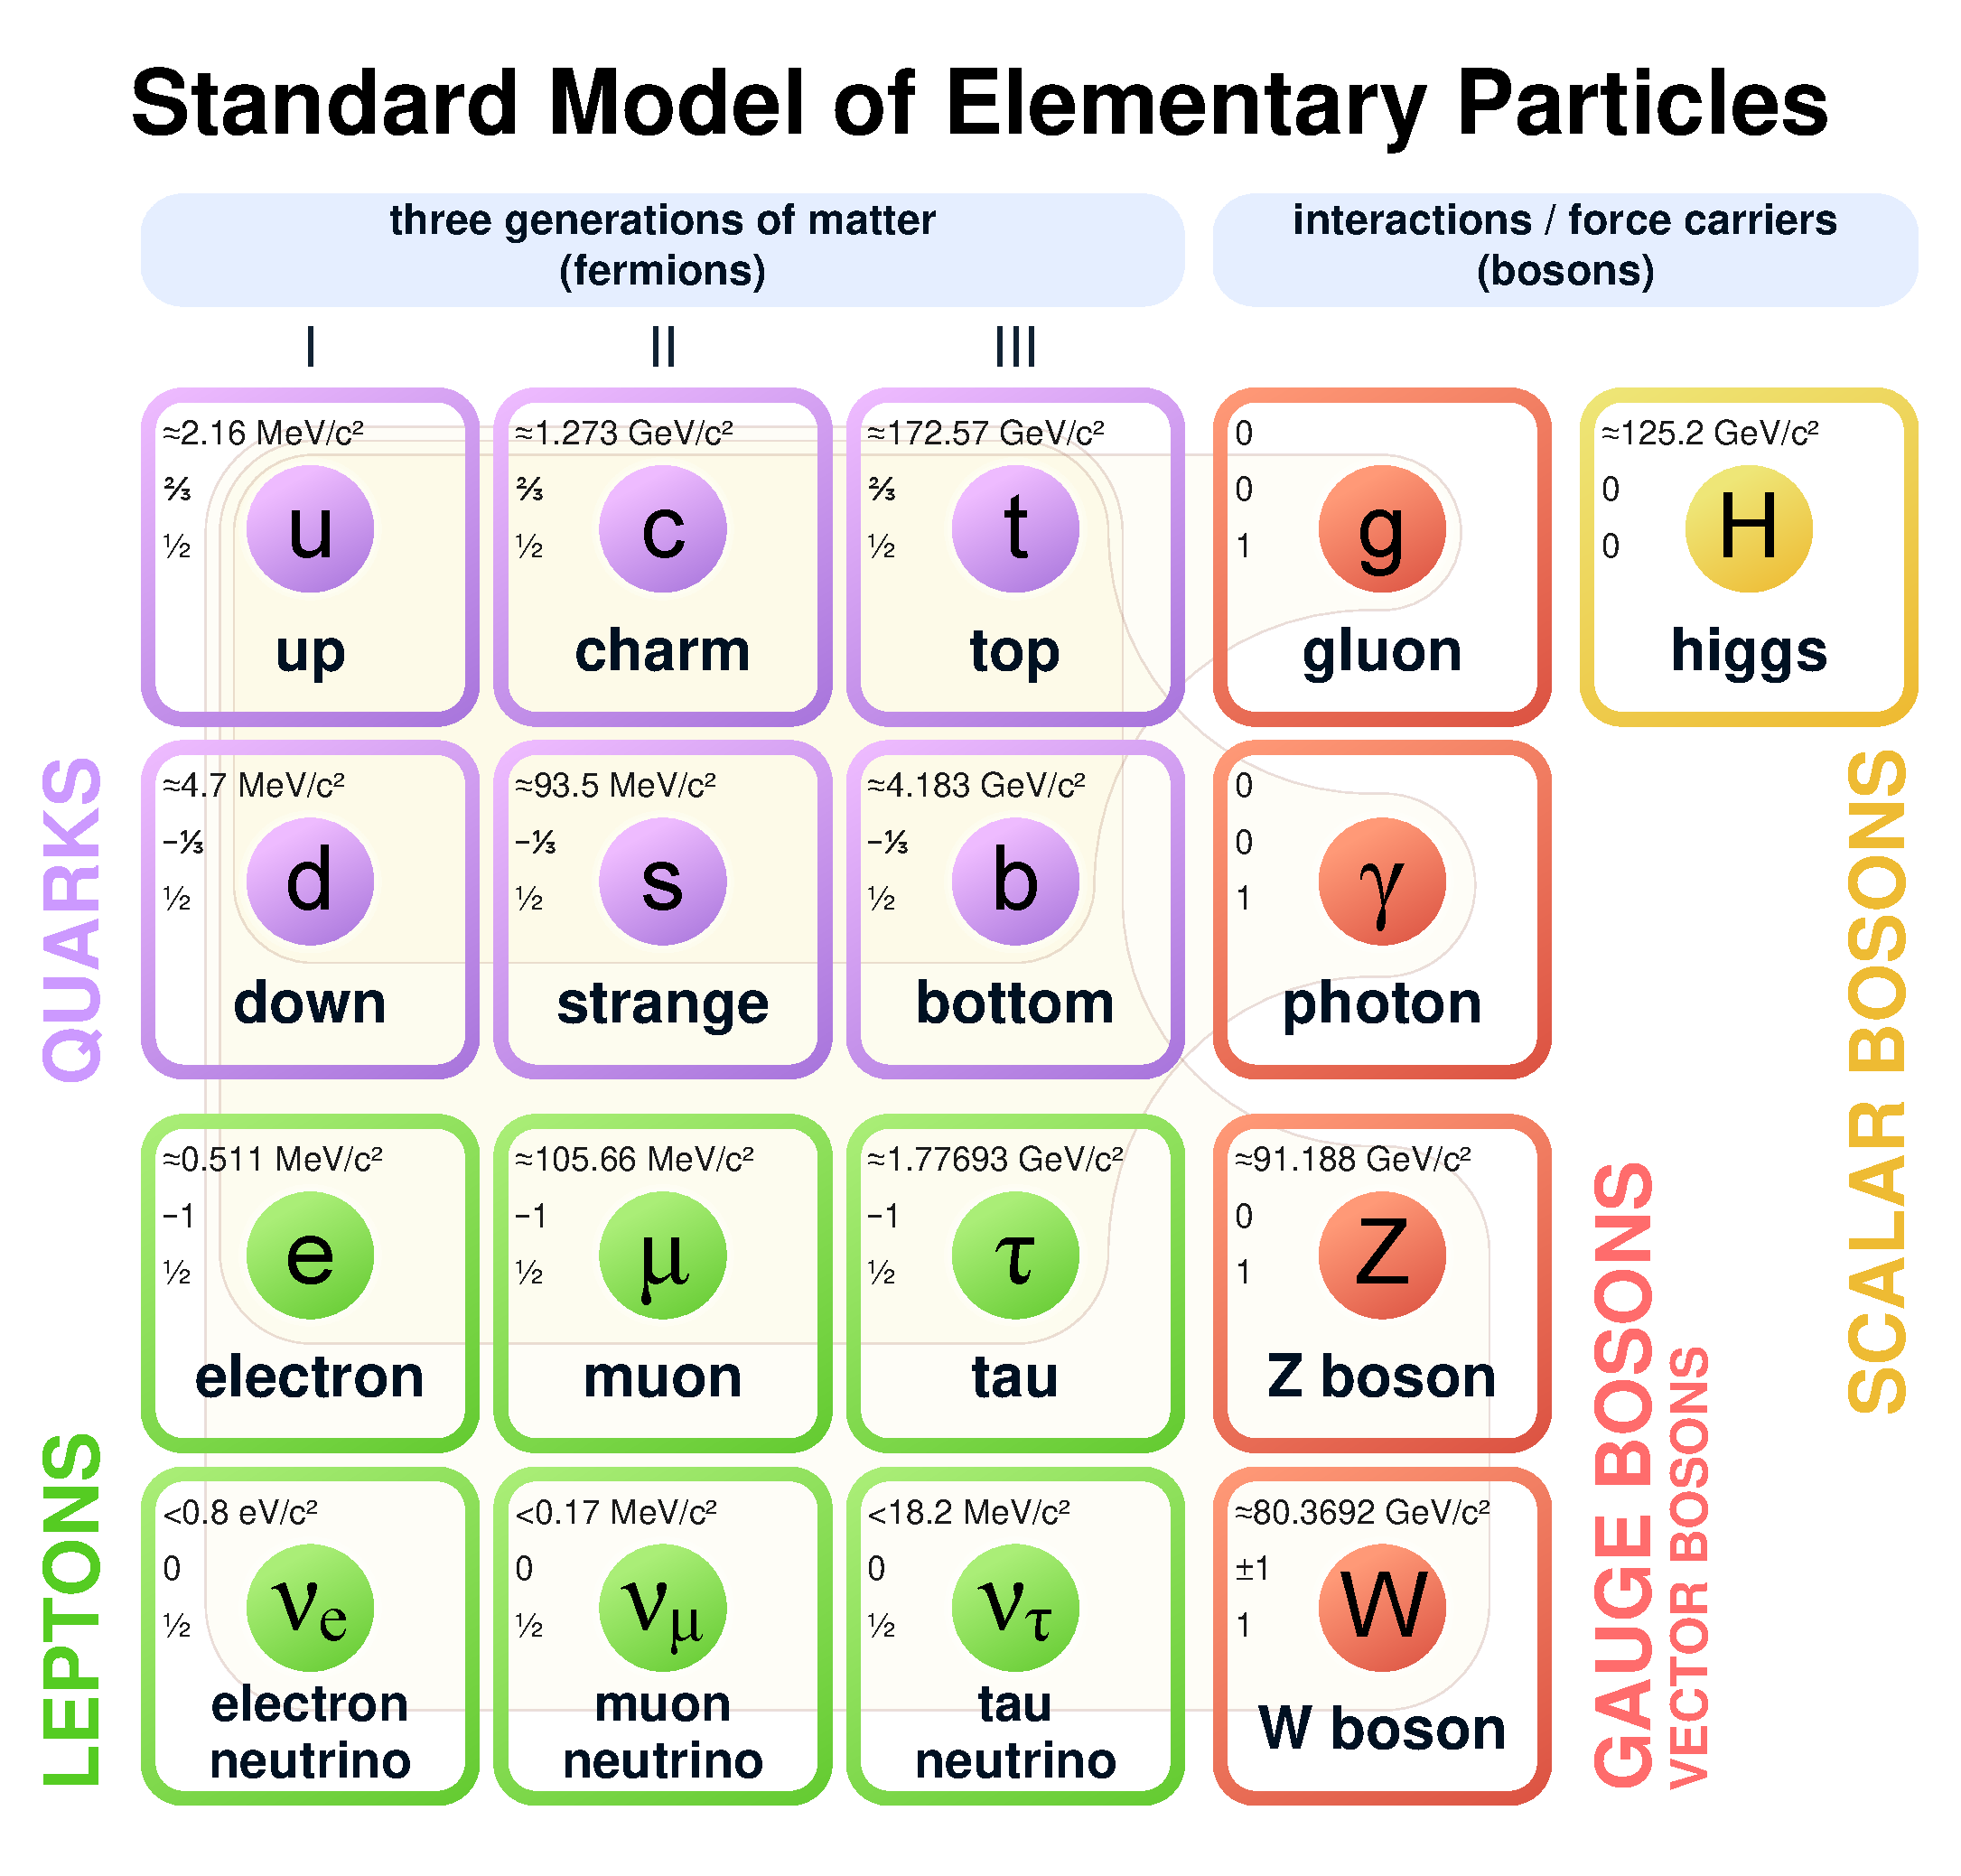
\includegraphics[width=10\baselineskip]{19_CosmicRayMuons/Standard_Model_of_Elementary_Particles.pdf}
\vspace{2em}
\end{center}
